\chapter{Realizacja}
W celu rozpoznania przechodnia został użyty połączony obraz termowizyjny i kolorowy nazywany dalej RGBIR. Następnie ten obraz zostaje poddany analizie HOG oraz klasyfikacji za pomocą SVM. W celu ustalenia obszaru zainteresowania na obrazie termowizyjnym za pomocą wzorca probabilistycznego zostają wytypowani kandydaci.

\section{Akwizycja obrazu}
Obraz kolorowy służy jako obraz bazowy. Rozdzielczości 640 x 480 pikseli, prędkością 30 klatek na sekundę i głębi 8 bitów na kanał. Źródłem tego obrazu jest kamera podłączona do układu za pomocą interfejsu HDMI. Na obraz bazowy zostaje nałożony obraz termowizyjny z kamery Lepton, który różni się znacząco parametrami. Abu je zsynchronizować zastosowano bufor ramki, do którego jest zapisywany obraz z prędkością 9 klatek na sekundę a odczytywany z prędkością 30. Kolejnym przekształceniem jest transformacja projekcyjna. Ma na celu powiększenie i dopasowanie obrazu by poprawnie pokrywał się z obraz wizyjnym. W tym celu został zaimplementowany moduł który oblicza na podstawie parametrów macierzy transformaty i koordynatami piksela obrazu źródłowego odpowiadającą mu pozycję na obrazie termowizyjnym zapisanym w buforze ramki. Następny moduł dokonuje interpolacji dwuliniowej. Do poprawnej interpolacji wymagane są 4 piksele otaczające obliczony z projekcji punkt. W celu zredukowania liczby dostępów do pamięci i zwiększenie szybkość działania moduł zapamiętuje 4 ostatnio użyte wartości pikseli. Rozwiązanie to pozwala na pracę w czasie rzeczywistym małym kosztem zasobów układu.
Strumień wizyjny jak i termowizyjny działają w AXI-Stream. Umożliwia to łatwą synchronizację obu obrazów na podstawie sygnału SOF (ang. Start o frame). Moduł synchronizacji czeka na pojawienie się tego sygnału w strumieniu termowizyjnym. Do tego momentu wszystkie napływające piksele są odrzucane. Gdy pojawi się sygnał strumień IR zostaje zatrzymany i czeka na pojawienie się sygnału SOF w bazowym strumieniu wizyjnym. Po jego wykryciu strumień IR rusza. Oba strumienie zostają zsynchronizowane tworząc strumień wizyjna obrazu RGBIR. Następnie ten strumień zostaje przesłany do pamięci za pośrednictwem VDMA oraz (po koloryzacji i nałożeniu) wyświetlony na monitorze przez port VGA.

\section{Wyznaczanie ROI}
Strumień IR z kamery zostaje zbinearyzowany i zbadany w detektorze DPM. Moduł DPM przesyła do pamięci listę koordynatów kandydatów wraz z mocą dopasowania. Moduł DPM został zaczerpnięty z pracy inżynierskiej. Moduł wykorzystuję strumień bezpośrednio z kamery. Wielkość okna detekcji wynosi 16 x 40 pikseli. Jeżeli badany obraz binarny wykazał odpowiedni poziom dopasowania do wzorca zostaje wysłana o tym informacja poprzez AXI-Stream do pamięci. Informacja zawiera koordynaty okna w układzie odniesienia kamery IR oraz wartość mocy dopasowania. Gdy zostanie zbadane ostatnie okno w obrazie zostaje wysłany sygnał LAST co wygeneruje przerwanie dla systemu procesorowego.

\section{Klasyfikacja za pomcą SVM}
Z lisy kandydatów wygenerowanej przez moduł DPM wybierany jest wynik o najwyższej mocy dopasowania. Koordynaty z układu odniesienia kamery zostają poddane transformacie projekcyjnej do układu odniesienia kamery RGB. Z obszaru na obrazie RGBIR zawierającym potencjalnie człowieka zostają wyodrębnione cechy HOG które następnie służą jako wektor dla SVM.

Klasyfikator został opracowany i nauczony na podstawie 60 wyselekcjonowanych obrazów. 30 z nich stanowiło próbką pozytywną zawierającą osobę a 30 nie. Nauczanie zostało zrealizowane przy użyciu oprogramowania Matlab. Próbki pozytywne zostały wygenerowane poprzez zapis ROI wyznaczonych przez wzorzec probabilistyczny. 

\section{Prezentacja wyników}
Na wyjściu konsoli zostają podane współrzędne oraz moc dopasowania i klasyfikacja obiektu. Na obrazie wyjściowym VGA obszar ten zostaje zaznaczony zieloną ramką. Jeżeli potencjalny obszar nie został zakwalifikowany jako człowiek ale miał największą moc dopasowania DPM to obszar zostaję zaznaczony czerwoną ramką. Czarna ramka oznacza że nie został wykryty żaden obiekt. 

Mając do dyspozycji układ heterogeniczny rodziny Zynq-7000 od firmy Xilinx operacje zostały podzielone między programowalną logiką a systemem procesorowym. Ogólny zarys systemu został przedstawiony na rysunku \ref{fig:systemwizyjny}.

\begin{figure}[h]
    \centering
    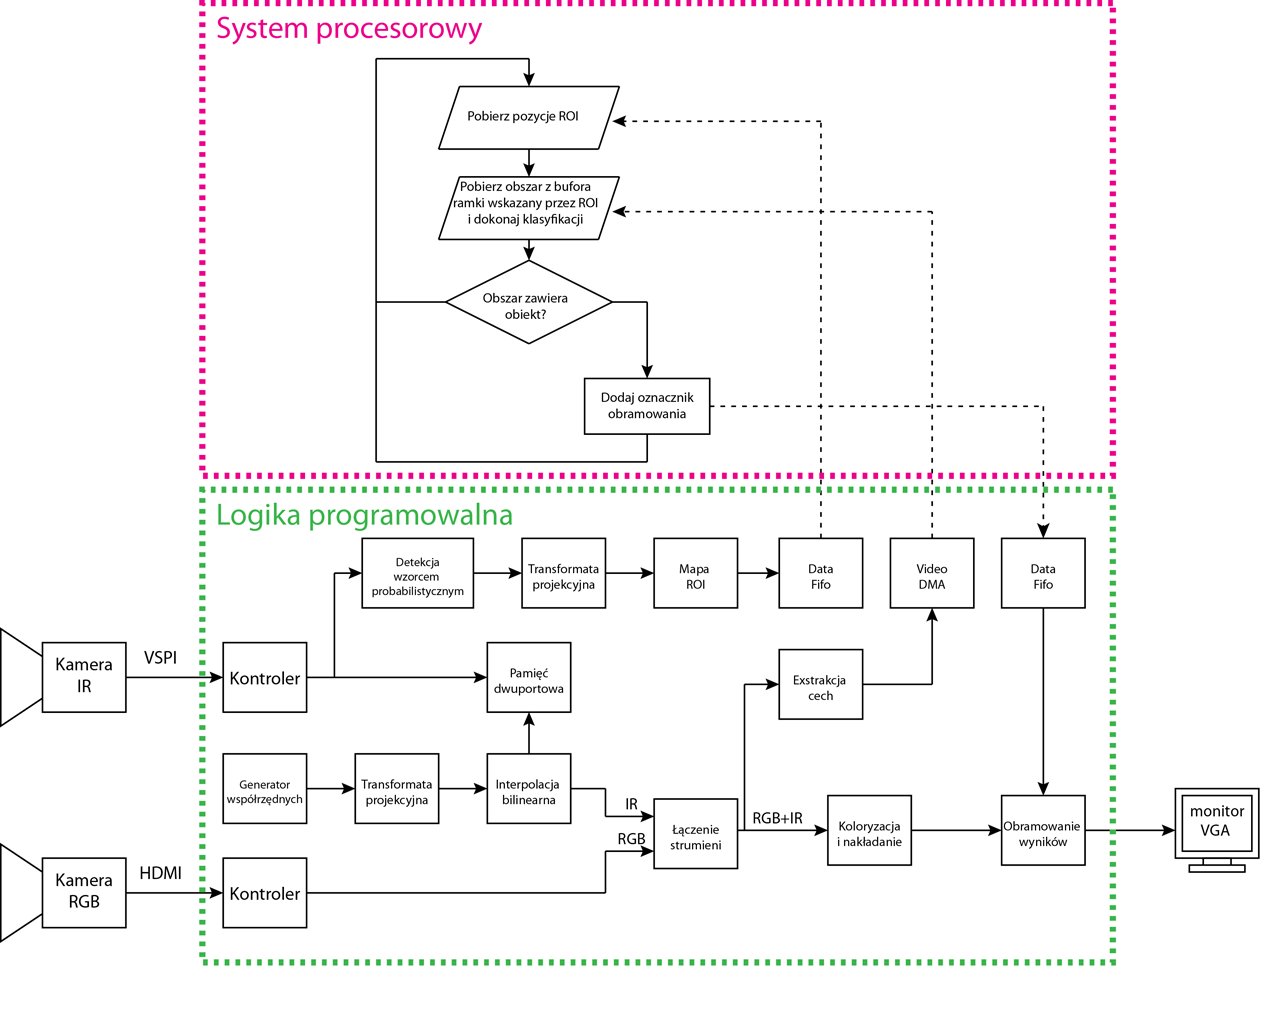
\includegraphics[width=1\textwidth]{images/system}
    \caption{Schemat blokowy systemu detekcji.}
    \label{fig:systemwizyjny}
\end{figure}

Programowalna logika:
\begin{itemize}
\item Akwizycja Obrazu poprzez HDMI (RGB) i VoSPI (IR),
\item Transformata projekcyjna i interpolacja obrazu IR,
\item Nałożenie i synchronizacja obrazu IR do obrazu RGB,
\item Prezentacja wyników,
\item Detekcja kandydatów za pomocą wzorca probabilistycznego.
\end{itemize}
System Procesorowy:
\begin{itemize}
\item konfiguracja parametrów systemu wizyjnego w logice programowalnej poprzez interfejs AXI-Lite,
\item Klasyfikacja obszarów wytypowanych przez wzorzec probabilistyczny,
\item Generowanie oznaczników.
\end{itemize}

\section{Opis modułów}
\subsection{Kontroler kamery IR}
Pobiera obraz z kamery poprzez interfejs VoSPI który następnie zostaje zapisany do dwuportowej pamięci BRAM. 
\subsection{Transformata projekcyjna}
Zadaniem modułu jest dostosowanie obrazu IR by pokrywał się z obrazem RGB. Moduł transformaty projekcyjnej zamienia wygenerowane współrzędne w zakresie wielkości przychodzącego obrazu RGB na odpowiadające im punkt na obrazie IR (wraz z częścią ułamkową). Moduł jest konfigurowalny poprzez interfejs AXI-Lite, za pomocą którego można ustawić wartość minimalną i maksymalną współrzędnych wyjściowych U i V oraz macierz transformaty.
\subsection{Interpolacja bilinearna}
Prosty moduł przeznaczony głównie do powiększania obrazów. Pobiera wartość 4 otaczających, podanych na wejściu punktu, pikseli z BRAM i na ich bazie jest wykonywana interpolacja. Moduł zapamiętuje 4 ostatnio użyte piksele które są na bieżąco aktualizowane wraz z zmianą położenia punktu wejściowego na obrazie IR.
\subsection{Łączenie strumieni}
Moduł posiada dwa wejścia dla obrazu. Jeden strumień jest głównym i do niego jest dołączany drugi strumień. Do synchronizacja strumieni została wykorzystana możliwość AXI-Strem do wstrzymania transmisji. Piksele z dołączanego strumienia są odrzucane do momentu pojawienia się sygnału SOF. W momencie pojawienia się sygnału SOF w strumieniu głównym transmisja zostaje wznowiona pod kontrolą strumienia wyjściowego. 
\subsection{Koloryzacja i nakładanie}
Połączone strumienie RGB+IR zostają połączone w jeden obraz. Obraz IR zostaje poddany koloryzacji na podstawie 12-bitowego LUT i nałożony w proporcjach 50 na 50 z obrazem RGB.
